\section{Solution}
In this section we describe the key ideas behind our design, and the decisions we made during the design process.
\subsection{Idea}

Figure ~\ref{fig:architecture} shows an architecture diagram of our design.

To store the last 4 input values for each of the streams,  we allocate 4 arrays of size $n$ in BRAM. When input is ready we move the contents of the $i^{th}$ array to the $(i+1)^{th}$ for $0 \leq i < 4$, and store the input value corresponding to $j{^th}$ stream to the $j^{th}$ block of array 0. The filtering happens as follows. For $0 \leq  i < n$ and $0 \leq j < 4$ we load the $i^{th}$ value from the $j^{th}$ array from the input buffer arrays.  These 4 values are used as input values for the FIR, together with the corresponding coefficients according to the direct equation for the filter. The values from the array are requested one clock cycle before they are needed in the computation, since reads in the BRAM are performed synchronously. As seen in the diagram, we use 4 multipliers in parallel. Alternatively we could have used one multiplier doing 4 sequential operations for each sample, but we decided to optimize for throughput and not for hardware usage.

The coefficients $h[]$ are the same as in lab L4 and because they are symmetric we store only $2L+1$ of them.

The input storing and FIR processing for each stream happens in the same clock cycle, so that we could theoretically produce one output per clock cycle.
\begin{figure}
\begin{center}
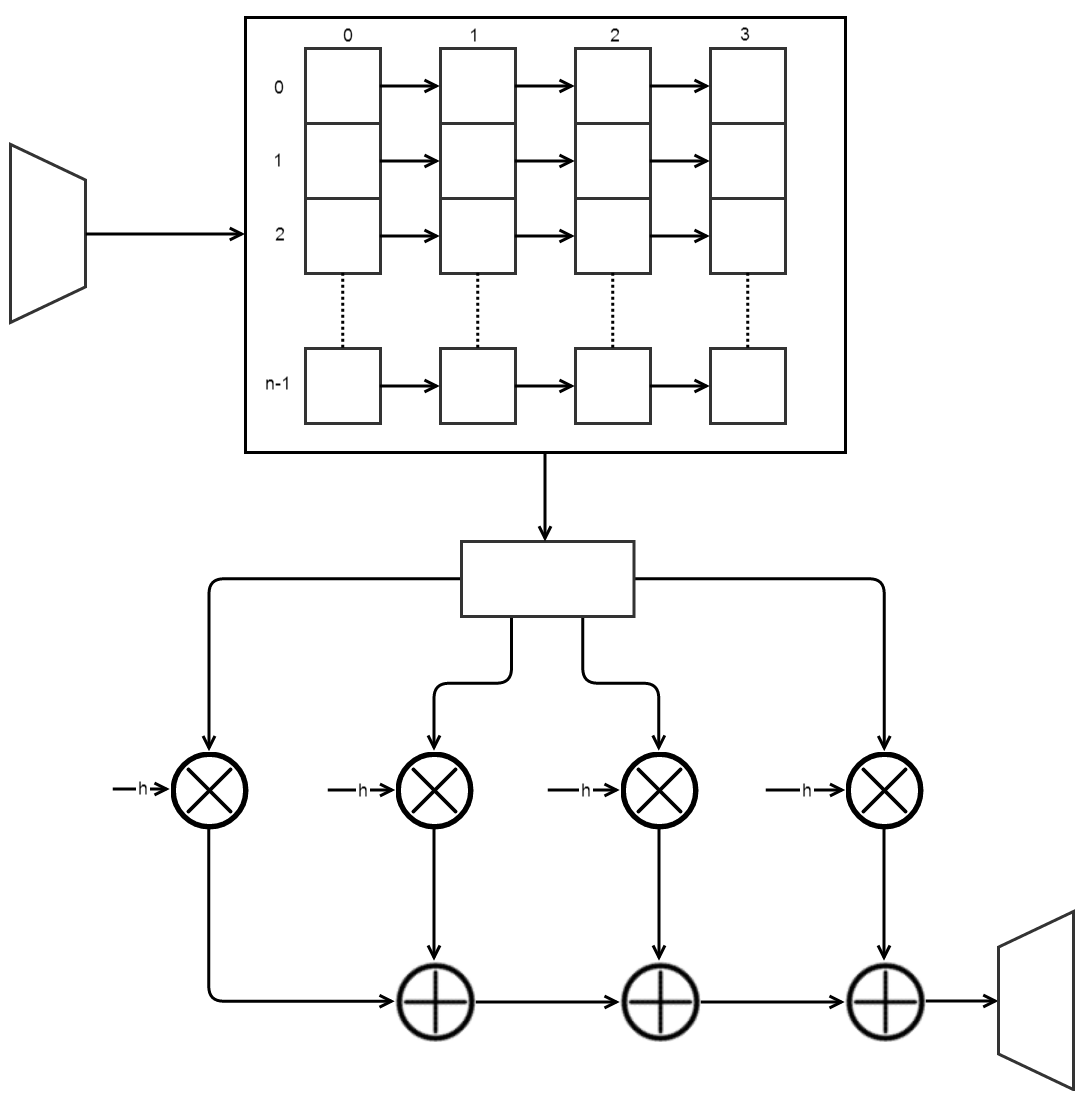
\includegraphics[width=0.7\textwidth]{images/architecture.png}
\caption{Architecture diagram of the system.}
\label{fig:architecture}
\end{center}
\end{figure}

\subsection{Implementation}
